\documentclass[11pt]{article}

%Menge: \mathbb{R}

\usepackage[ngerman]{babel}
\usepackage{amsmath} %align, für = untereinander einfach &=
\usepackage{amssymb}
\usepackage{amsthm}
\usepackage{listings}
\usepackage[utf8]{inputenc}
\usepackage{graphicx}
\usepackage{esvect}
\graphicspath{ {./images/} }
\usepackage{tikz}         % For arrow and dots in \xvec
\usepackage[left=2.30cm, right=2.30cm, top=1.70cm, bottom=2.00cm]{geometry}

% --- Macro \xvec
\makeatletter
\newlength\xvec@height%
\newlength\xvec@depth%
\newlength\xvec@width%
\newcommand{\xvec}[2][]{%
	\ifmmode%
	\settoheight{\xvec@height}{$#2$}%
	\settodepth{\xvec@depth}{$#2$}%
	\settowidth{\xvec@width}{$#2$}%
	\else%
	\settoheight{\xvec@height}{#2}%
	\settodepth{\xvec@depth}{#2}%
	\settowidth{\xvec@width}{#2}%
	\fi%
	\def\xvec@arg{#1}%
	\def\xvec@dd{:}%
	\def\xvec@d{.}%
	\raisebox{.2ex}{\raisebox{\xvec@height}{\rlap{%
				\kern.05em%  (Because left edge of drawing is at .05em)
				\begin{tikzpicture}[scale=1]
				\pgfsetroundcap
				\draw (.05em,0)--(\xvec@width-.05em,0);
				\draw (\xvec@width-.05em,0)--(\xvec@width-.15em, .075em);
				\draw (\xvec@width-.05em,0)--(\xvec@width-.15em,-.075em);
				\ifx\xvec@arg\xvec@d%
				\fill(\xvec@width*.45,.5ex) circle (.5pt);%
				\else\ifx\xvec@arg\xvec@dd%
				\fill(\xvec@width*.30,.5ex) circle (.5pt);%
				\fill(\xvec@width*.65,.5ex) circle (.5pt);%
				\fi\fi%
				\end{tikzpicture}%
	}}}%
	#2%
}

%eigene Befehle:
\newcommand{\R}{$\mathbb{R}$}


\title{Blatt 6} %% Template in den entsprechenden Namen ändern


\begin{document}
\lstset{language=Java}
\author{Tom Herrmann}
\date{\today}
\maketitle
\section{Aufgabe 1}
\section{Aufgabe 2}
\subsection{a}
\begin{center}
	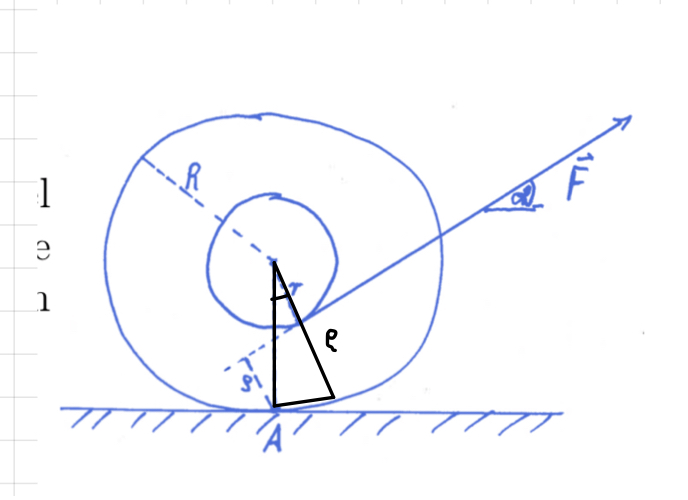
\includegraphics[scale= 0.3]{IMG_E710CED3176C-1.jpeg}
\end{center}
Aus dem eingezeichneten Dreieck kann man die Beziehung direkt ablesen und ist damit recht offensichtlich.
\subsection{b}
\begin{align*}
	cos \alpha ? \frac{r + \rho}{R}\\
	-\vec{M} = \vec{r} \times \vec{F} \qquad |\vec{M}| = |\vec{r}| |\vec{F}| sin \varphi\\
	M = \rho \cdot F = 0\\
\end{align*}
\section{Aufgabe 3 }
	Von der ERde zum Mars
	\subsection{a}
		\begin{align*}
			I = mr^2 \qquad \vec{L} = I \vec{w}; |\vec{L}| = Iw\\
			E_{rot}= I \frac{w^2}{2} = \frac{L^2}{2I}
		\end{align*}
\section{Aufgabe 4}
	\subsection{a}
		\begin{align*}
			E_{oot} = Gm\left( \frac{M_s}{r_p} + \frac{M_p}{R_p} \right)
		\end{align*}
		wobei das Trägheitsmoment für die Erde dann:
		\begin{align*}
			I_E = M_E r_E^2 \text{ und } E_{rot, E} = \frac{1}{2} I_E w_E^2
		\end{align*}
Man kann nun durch das Kräftegleichtgewicht weiter rechnen welches zwischen Sonne und Sonne wirkt.
	 \[M_E r_e w_E^2 = G \frac{M_S M_E}{r_E^2}\]
	wobei sichdann $M_E$ rauskürzen lässt
	\[E_{rot,E} = \frac{1}{2} M_{E} r_{E}^2 G \frac{M_S}{r_{E}^3}\]
\subsection{b}
Man muss mal Drehmoment und Drehimpuls kompensireren.
$mw^2 R = mg = R = 
\frac{g}{w^2} , \qquad W = \frac{2 \pi}{30s} = 0.2094395102$  
\subsection{c}
\begin{align*}
	E_{rot,L} = \frac{1}{2} mR^2 w^2\\
	E_{rot, 2} = 0 \qquad A = E_{rot , 1}
\end{align*}
Corioliskraft lassen wir außenvor da wir auf diese keine Arbeit verrichten. Dies folgt aus der Definition der Corioliskraftn also dass diese senkrecht wirkt...

\section{Aufgabe 5}
	\[ m \ddot{x} = - v^\prime (x) \]
	\begin{align*}
		E = \frac{1}{2} m \dot{x}^2 + v(x) &= const\\
		\frac{d}{dt} (E) = m\ddot{x} \dot{x} + v^\prime (x) \dot{x} &= \dot{x} (m \ddot{x} + v^\prime(x))\\\\
		E = \frac{1}{2} m \dot{x}^2 + v(x) = const \qquad \dot{x}^2 = \frac{2}{m} (E - v(x))\\
		\text{wobei } \dot{x} = \sqrt{\frac{2}{m} (E - V (x))}\\
		\int\limits_{a}^{b} \frac{dx}{\dot{x}} = \int\limits_{a}^{b}\frac{dx}{\sqrt{\frac{2}{m} (e- v(x))}}\\\\
		T = \int\limits_{a}^{b} dx \frac{(E-v(x)))}{2m}^{-\frac{1}{2}}
  	\end{align*}
  	
  	\section{Aufgabe 6}
  \textbf{ Definitionen für die Aufgabe}
  	\begin{align}
  		\mu = \frac{m_1 m_2}{m_1 + m_2}\\
  		\vec{r} = \vec{r}_1 - \vec{r}_2\\
  		\vec{R} = \frac{m_1 \vec{r}_1 + m_1 \vec{r_2}}{m_1 + m_2}
  	\end{align}
  	\textbf{Rechnung:}
  	\begin{align*}
  		m_1 \vec{r}_1 \times \dot{\vec{r}}_1 + m_2 \vec{r}_2 \times \dot{\vec{r}}_2\\
  		&=(m_1 + m_2) \vec{R} \times \dot{\vec{R}} + \mu \vec{r} \times \dot{\vec{r}}\\
  		&= \frac{1}{m_1 + m_2} \left[ (m_1\vec{r}_1 + m_2 \vec{r}_2) \times ( m_1 \dot{\vec{r}}_1 + m_2 \dot{\vec{r}}_2 ) + m_1 m_2 (\vec{r}_1 - \vec{r}_2) \times (\dot{\vec{r}}_1 - \dot{\vec{r}}_2 )   \right]\\
  		  	\end{align*}
  		\[ = \frac{1}{m_1+m_2}\left[ m_1^2 \vec{r}_1 \times \dot{\vec{r}}_1 + m_1 m_2 \vec{r}_1 \times \dot{\vec{r}}_2 + m_1 m_2 \vec{r}_2 \times \dot{\vec{r}}_1 + m_1^2 \vec{r}_2 \times \dot{\vec{r}}_2 + m_1 m_2 \vec{r}_1 \times \dot{\vec{r}}_1 - m_1 m_1 \vec{r}_1 \times \dot{\vec{r}}_2\] \[- m_1 m_2 \vec{r}_2 \times \dot{\vec{r}}_1 + m_1 m_2 \vec{r}_2 \times \dot{\vec{r}}_2 \right] \]
  	Nun kürzen sich aus dem ganzen auspultiplizierten ein paar Dinge heraus
  	\[ \frac{1}{m_1 + m_2} \left[ (m_1^2 + m_1m_2)\vec{r}_1 \times \dot{\vec{r}}_1  + (m_2^2 + m_1m_2) \vec{r}_2 \times \dot{\vec{r}}_2  \right] \]
\end{document}




